\section{Statistics of the initial perturbations}
\label{sec:statistics_of_the_initial_perturbations}

Having introduced the governing equations in \cref{sec:governing_equation}, we now turn our attention to the statistical description of the initial conditions. Our objective is to relate their spatial covariance to a physically realizable perturbation that can be imposed in a controlled experiment or numerical simulation. In fact, one contribution made here is to overcome an apparent limitation in the formulation introduced by \citet{frame-towne-2024} for Poiseuille flow, where the initial covariance was treated primarily as a mathematical model and did not necessarily correspond to a directly measurable experimental quantity. Here, instead, we show that the methodology is considerably more general and that the initial correlation has a precise physical meaning.

In physical space, the covariance of the initial perturbation field is
\begin{equation}
    \mathsfbi{C}_{00}(\boldsymbol{x},\boldsymbol{r})
    =
    \mean{
        \boldsymbol{q}'(\boldsymbol{x}),
        \boldsymbol{q}'(\boldsymbol{x}+\boldsymbol{r})
    }
    =
    \begin{pmatrix}
        C_{00}^{ww}(\boldsymbol{x},\boldsymbol{r})
        &
        C_{00}^{w\rho}(\boldsymbol{x},\boldsymbol{r})
        \\[4pt]
        C_{00}^{\rho w}(\boldsymbol{x},\boldsymbol{r})
        &
        C_{00}^{\rho\rho}(\boldsymbol{x},\boldsymbol{r})
    \end{pmatrix}.
    \label{eq:physical_covariance_general}
\end{equation}
For the initial conditions that we wish to describe here, we assume that they can be represented through a perturbation of the interface separating the two fluids \citep{cook-dimotakis-2001,wei-livescu-2012}, and that they are homogeneous and isotropic. In principle, this is not the only possibility, since the disturbance may also be introduced through the vertical velocity, as discussed by \citet{mueschke-schilling-2009}, and need not necessarily be isotropic \citep{dalziel-linden-youngs-1999}. Even though these assumptions do not encompass all possible initial conditions that may arise in experiments or numerical initializations, they still provide a physically relevant setting that captures the fundamental nature of the problem, as reflected by the large number of studies that have adopted them \citep{kord-capecelatro-2019}; moreover, the framework that we develop can readily accommodate more general prescriptions. The hypotheses we adopt are intended solely to keep the exposition clear from additional cumbersome notations, without sacrificing the physical interpretation of the prescribed statistics of the initial conditions. Under these assumptions, the initial vertical-velocity perturbation is set to zero, so that all covariance components involving \(w\) vanish and only the density-density component remains nonzero, namely
\begin{equation}
    \mathsfbi{C}_{00}(\boldsymbol{x},\boldsymbol{r})
    =
    \mean{
        \boldsymbol{q}'(\boldsymbol{x}),
        \boldsymbol{q}'(\boldsymbol{x}+\boldsymbol{r})
    }
    =
    \begin{pmatrix}
        0 & 0
        \\[4pt]
        0 & C_{00}^{\rho\rho}(\boldsymbol{x},\boldsymbol{r})
    \end{pmatrix}.
    \label{eq:physical_covariance_density_only}
\end{equation}
Denoting the horizontal coordinate by \(\boldsymbol{x}_h=(x,y)\) and the local displacement of the interface by \(\eta(\boldsymbol{x}_h)\), the displaced base density profile admits the expansion
\begin{equation}
    \rho_0(z-\eta)
    =
    \rho_0(z)
    -
    \rho_{0,z}(z)\,\eta(\boldsymbol{x}_h)
    +
    O\!\left(\eta^2\right).
    \label{eq:initial_density_displacement}
\end{equation}
Consequently, at leading order, the initial density perturbation is determined directly by the local displacement of the base density profile according to
\begin{equation}
    \rho'(\boldsymbol{x},0)
    =
    -
    \rho_{0,z}(z)\,\eta(\boldsymbol{x}_h).
    \label{eq:initial_density_perturbation_eta}
\end{equation}
Substitution of \eqref{eq:initial_density_perturbation_eta} into the density covariance then gives
\begin{equation}
    C_{00}^{\rho\rho}(\boldsymbol{x}_h,\boldsymbol{r}_h,z,z')
    =
    \underbrace{
        \rho_{0,z}(z)\,\rho_{0,z}(z')
    }_{
        C_{00}^{z}(z,z')
    }
    \underbrace{
        \mean{
            \eta(\boldsymbol{x}_h)
            \eta(\boldsymbol{x}_h+\boldsymbol{r}_h)
        }
    }_{
        C_{00}^{xy}(\boldsymbol{x}_h,\boldsymbol{r}_h)
    }.
    \label{eq:initial_density_covariance_separable}
\end{equation}
Equation \eqref{eq:initial_density_covariance_separable} separates the initial density covariance into two physically distinct contributions. The vertical factor is determined entirely by the base state, whereas the horizontal factor contains the prescribed statistics of the interface displacement. In particular, \(C_{00}^{z}\) is fixed by \(\rho_{0,z}\) and retains the inhomogeneity of the diffusive layer, so that the initial perturbations are localized within this layer and their vertical correlation length is associated with its initial thickness. For the diffusive profile considered here, the vertical covariance factor is
\begin{equation}
    C_{00}^{z}(z,z')
    =
    \frac{4\,\Atw^{2}}{\pi\,\delta_0^{2}}
    \exp\!\left(
        -\frac{z^2+{z'}^2}{\delta_0^2}
    \right).
    \label{eq:vertical_covariance_factor_erf}
\end{equation}
The horizontal correlation \(C_{00}^{xy}\), on the other hand, carries the statistical information associated with the displacement of the interface and, although this correlation may be prescribed directly in physical space, perturbations imposed experimentally or numerically are often characterized more naturally through their spectral content; this is where we draw a direct connection between the statistical description of the perturbations and the classical spectra used to initialize direct numerical simulations \citep{rogallo-1981}.


Since the perturbation field is homogeneous in the horizontal plane, we write
\begin{equation}
    \eta(\boldsymbol{x}_h)
    =
    \int_{\mathbb{R}^2}
        \hat{\eta}(\boldsymbol{k}_h)
        \exp(i\boldsymbol{k}_h\bcdot\boldsymbol{x}_h)
    \,\mathrm{d}\boldsymbol{k}_h,
    \qquad
    \boldsymbol{k}_h=(k_x,k_y).
    \label{eq:eta_fourier_transform}
\end{equation}
The corresponding spectral density \(\Phi_{00}^{xy}\) is defined by
\begin{equation}
    \mean{
        \hat{\eta}(\boldsymbol{k}_h)
        \hat{\eta}^{\ast}(\boldsymbol{k}'_h)
    }
    =
    \Phi_{00}^{xy}(\boldsymbol{k}_h)
    \delta(\boldsymbol{k}_h-\boldsymbol{k}'_h),
    \label{eq:eta_spectral_density_definition}
\end{equation}
so that the physical-space correlation is obtained as the Fourier transform of the spectral density,
\begin{equation}
    C_{00}^{xy}(\boldsymbol{r}_h)
    =
    \int_{\mathbb{R}^2}
        \Phi_{00}^{xy}(\boldsymbol{k}_h)
        \exp(i\boldsymbol{k}_h\bcdot\boldsymbol{r}_h)
    \,\mathrm{d}\boldsymbol{k}_h.
    \label{eq:eta_correlation_spectral_density}
\end{equation}
Invoking the isotropy assumption introduced above, the correlation depends only on \(r=\lvert\boldsymbol{r}_h\rvert\), while the spectral density depends only on \(k=\lvert\boldsymbol{k}_h\rvert\), and therefore
\begin{equation}
    C_{00}^{xy}(r)
    =
    2\pi
    \int_0^\infty
        \Phi_{00}^{xy}(k)
        J_0(kr)\,
        k
    \,\mathrm{d}k,
    \label{eq:eta_correlation_hankel_phi}
\end{equation}
where
\begin{equation}
    J_0(kr)
    =
    \frac{1}{2\pi}
    \int_0^{2\pi}
        \exp(i k r\cos\theta)
    \,\mathrm{d}\theta
    \label{eq:bessel_j0}
\end{equation}
is the Bessel function of the first kind of order zero. The two-dimensional isotropic spectrum of the interface displacement is then defined as the circularly integrated spectral density
\begin{equation}
    E_{\eta}(k)
    =
    \pi k\,\Phi_{00}^{xy}(k),
    \label{eq:eta_2d_spectrum_definition}
\end{equation}
with the normalization chosen such that
\begin{equation}
    \mean{\eta_0^2}
    =
    2
    \int_0^\infty
        E_{\eta}(k)
    \,\mathrm{d}k.
    \label{eq:eta_variance_spectrum}
\end{equation}
It is immediate to show that the in-plane correlation and the isotropic spectrum form the Hankel transform pair
\begin{equation}
    C_{00}^{xy}(r)
    =
    2
    \int_0^\infty
        E_{\eta}(k)
        J_0(kr)
    \,\mathrm{d}k,
    \qquad
    E_{\eta}(k)
    =
    \frac{k}{2}
    \int_0^\infty
        C_{00}^{xy}(r)
        J_0(kr)\,
        r
    \,\mathrm{d}r.
    \label{eq:eta_hankel_transform_pair}
\end{equation}
This equivalence provides the desired connection between the two descriptions, since prescribing the correlation \(C_{00}^{xy}(r)\) in physical space is equivalent to prescribing the spectrum \(E_{\eta}(k)\) in Fourier space, with both representing the same random displacement of the interface. Consequently, modelling the spatial correlation is equivalent to imposing the corresponding spectrum when initializing the perturbations in a numerical simulation or controlled experiment.

\begin{figure}
    \centering
    \begin{minipage}{0.48\textwidth}
        \centering
        % This file was created by matlab2tikz.
%
\definecolor{mycolor1}{rgb}{0.48200,0.16500,0.51400}%
\definecolor{mycolor2}{rgb}{0.10600,0.47100,0.21600}%
\definecolor{mycolor3}{rgb}{0.68600,0.55300,0.76500}%
%
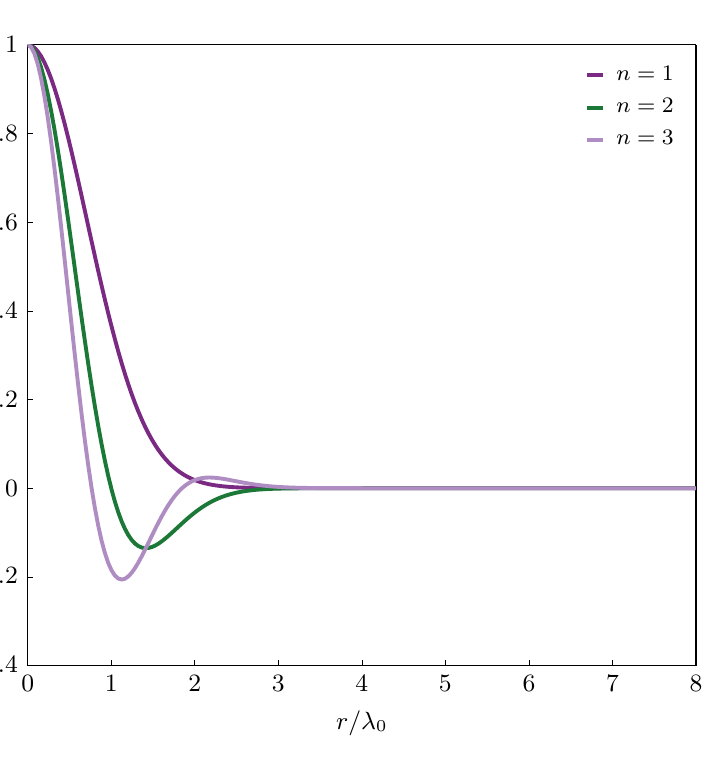
\begin{tikzpicture}[trim axis left,trim axis right]

\begin{axis}[%
width=11.252in,
height=7.131in,
at={(1.887in,0.962in)},
scale only axis,
clip=true,
separate axis lines,
every outer x axis line/.append style={black},
every x tick label/.append style={font=\color{black}},
every x tick/.append style={black},
xmin=0,
xmax=8,
xlabel={$r/\lambda_0$},
every outer y axis line/.append style={black},
every y tick label/.append style={font=\color{black}},
every y tick/.append style={black},
ymin=-0.4,
ymax=1,
ylabel={$C_{00,n}^{xy}(r)$},
axis background/.style={fill=white},
legend style={legend cell align=left, align=left},
clip=true,
clip mode=individual,
axis lines=box,
xtick pos=bottom,
ytick pos=left,
tick align=inside,
major tick length=2pt,
width=0.7\linewidth,
height=0.65\linewidth,
every axis/.append style={font=\fontsize{9}{9}\selectfont},xlabel style={font=\fontsize{9}{9}\selectfont},title style={font=\fontsize{9}{9}\selectfont},
legend style={font=\fontsize{8}{9}\selectfont,inner sep=1pt,row sep=1pt,column sep=2pt,nodes={scale=1.00},draw=none},legend image post style={xscale=0.35},
legend columns=1,
scaled x ticks=false,
tick label style={/pgf/number format/fixed,/pgf/number format/precision=2},
every x tick label/.append style={font=\fontsize{9}{9}\selectfont\color{black}},
every y tick label/.append style={font=\fontsize{9}{9}\selectfont\color{black}},
,,
colormap={sigmamap}{rgb(0.0000)=(0.0200,0.1880,0.3800); rgb(0.1000)=(0.0743,0.3456,0.5616); rgb(0.2000)=(0.1918,0.4980,0.7060); rgb(0.3000)=(0.3890,0.6708,0.8226); rgb(0.4000)=(0.7552,0.8682,0.9228); rgb(0.5000)=(0.9690,0.9689,0.9689); rgb(0.6000)=(0.9425,0.8044,0.7614); rgb(0.7000)=(0.8767,0.4910,0.4020); rgb(0.8000)=(0.7869,0.2866,0.2470); rgb(0.9000)=(0.6186,0.1239,0.1568); rgb(1.0000)=(0.4040,0.0000,0.1220)}
]
\addplot [color=mycolor1, line width=1.4pt]
  table[row sep=crcr]{%
1e-06	0.999999999999\\
0.0400210050025012	0.998399601164802\\
0.0800410100050025	0.993613914988808\\
0.120061015007504	0.985688746313652\\
0.160081020010005	0.974699624420412\\
0.200101025012506	0.960750604625268\\
0.240121030015008	0.943972627966267\\
0.280141035017509	0.924521475140297\\
0.32016104002001	0.902575359394744\\
0.360181045022511	0.878332210368438\\
0.400201050025012	0.852006706724764\\
0.440221055027514	0.823827119687516\\
0.484243060530265	0.79097308236634\\
0.524263065532766	0.759684729113178\\
0.564283070535268	0.727300616844434\\
0.604303075537769	0.6940701748391\\
0.64432308054027	0.660239763357353\\
0.684343085542771	0.626049737144811\\
0.724363090545273	0.59173174103289\\
0.764383095547774	0.557506276865767\\
0.804403100550275	0.523580573109958\\
0.844423105552776	0.490146780255911\\
0.884443110555278	0.457380506752258\\
0.924463115557779	0.425439701962636\\
0.96448312056028	0.39446388472475\\
1.00450312556278	0.364573708720333\\
1.04452313056528	0.335870849201984\\
1.08454313556778	0.308438189804935\\
1.12456314057028	0.282340283299189\\
1.16458314557279	0.257624056274803\\
1.20460315057529	0.234319724928809\\
1.24462315557779	0.212441887331191\\
1.28464316058029	0.191990756752799\\
1.32466316558279	0.172953500776418\\
1.36868517108554	0.153616030642925\\
1.40870517608804	0.137456156692945\\
1.44872518109055	0.122602894026061\\
1.48874518609305	0.109004923383705\\
1.52876519109555	0.096605170968143\\
1.56878519609805	0.0853421343566971\\
1.60880520110055	0.0751511263337177\\
1.64882520610305	0.0659654235207782\\
1.68884521110555	0.0577173101953688\\
1.72886521610805	0.0503390110203401\\
1.76888522111056	0.0437635094916467\\
1.80890522611306	0.0379252516972433\\
1.84892523111556	0.0327607374274328\\
1.88894523611806	0.0282090027635224\\
1.92896524112056	0.0242119999879278\\
1.96898524612306	0.0207148820077474\\
2.00900525112556	0.0176661994786927\\
2.04902525612806	0.0150180194791661\\
2.08904526113057	0.012725974944051\\
2.12906526613307	0.0107492541581323\\
2.16908527113557	0.00905053946678608\\
2.20910527613807	0.00759590402492638\\
2.25312728164082	0.00624120162348047\\
2.29314728664332	0.00520297616216849\\
2.33316729164582	0.00432358823816512\\
2.37318729664832	0.00358134108139998\\
2.41320730165083	0.00295703121831066\\
2.45322730665333	0.0024337446047919\\
2.49324731165583	0.00199665468359556\\
2.53326731665833	0.00163282555159215\\
2.57328732166083	0.00133102275996024\\
2.61330732666333	0.00108153366651469\\
2.65332733166583	0.000875998719344083\\
2.69334733666833	0.000707254577226614\\
2.73336734167084	0.000569189565086317\\
2.77338734667334	0.000456611620243819\\
2.81340735167584	0.000365128604090978\\
2.85342735667834	0.000291040629623266\\
2.89344736168084	0.000231243882767755\\
2.93346736668334	0.000183145288956025\\
2.97348737168584	0.000144587290025496\\
3.01350737668834	0.000113781944435656\\
3.05352738169085	8.92535403114787e-05\\
3.09354738669335	6.97889106716043e-05\\
3.1375693921961	5.3046498924736e-05\\
3.1775893971986	4.1199914486186e-05\\
3.2176094022011	3.18966278072457e-05\\
3.2576294072036	2.46151277540626e-05\\
3.2976494122061	1.89351297201011e-05\\
3.3376694172086	1.45192218940205e-05\\
3.37768942221111	1.1097554015231e-05\\
3.41770942721361	8.45512553019439e-06\\
3.45772943221611	6.42128164882296e-06\\
3.49774943721861	4.8610741519019e-06\\
3.53776944222111	3.66818845661831e-06\\
3.57778944722361	2.75917915890061e-06\\
3.61780945222611	2.06879295846269e-06\\
3.65782945722861	1.54619058659399e-06\\
3.69784946223112	1.15190824727759e-06\\
3.73786946723362	8.55424368192136e-07\\
3.77788947223612	6.33219404399189e-07\\
3.81790947723862	4.6723533522549e-07\\
3.85792948224112	3.43657646102901e-07\\
3.89794948724362	2.51956292962435e-07\\
3.93796949224612	1.84133698326139e-07\\
3.97798949724862	1.34137500465833e-07\\
4.02201150275138	9.43196276680939e-08\\
4.06203150775388	6.82492105497248e-08\\
4.10205151275638	4.92268508511979e-08\\
4.14207151775888	3.53928342989794e-08\\
4.18209152276138	2.53651537421737e-08\\
4.22211152776388	1.8120430961328e-08\\
4.26213153276638	1.29035263483008e-08\\
4.30215153776888	9.1591921633164e-09\\
4.34217154277139	6.48059372303923e-09\\
4.38219154777389	4.57068496023989e-09\\
4.42221155277639	3.21333975834547e-09\\
4.46223155777889	2.25185734354156e-09\\
4.50225156278139	1.57301899928504e-09\\
4.54227156778389	1.09530716668187e-09\\
4.58229157278639	7.60233070441163e-10\\
4.62231157778889	5.2597663614046e-10\\
4.6623315827914	3.6273963865497e-10\\
4.7023515877939	2.49363247995418e-10\\
4.7423715927964	1.70875084877425e-10\\
4.7823915977989	1.16716943962175e-10\\
4.8224116028014	7.9469035013004e-11\\
4.8624316078039	5.39350192834225e-11\\
4.90645361330665	3.50836095281114e-11\\
4.94647361830916	2.36513420422409e-11\\
4.98649362331166	1.58933766667526e-11\\
5.02651362831416	1.06459747216356e-11\\
5.06653363331666	7.1082640536508e-12\\
5.10655363831916	4.73097378204817e-12\\
5.14657364332166	3.13867535609458e-12\\
5.18659364832416	2.07563564786554e-12\\
5.22661365332666	1.36824765173743e-12\\
5.26663365832917	8.99056880984078e-13\\
5.30665366333167	5.88868731658669e-13\\
5.34667366833417	3.84466661568461e-13\\
5.38669367333667	2.50211776318582e-13\\
5.42671367833917	1.62317622470872e-13\\
5.46673368334167	1.04962089263502e-13\\
5.50675368834417	6.76562820137053e-14\\
5.54677369334667	4.34703018874741e-14\\
5.58679369834918	2.78410783066888e-14\\
5.62681370335168	1.77741284597066e-14\\
5.66683370835418	1.13109594300301e-14\\
5.70685371335668	7.17495930073217e-15\\
5.74687371835918	4.53678612841743e-15\\
5.79089572386193	2.73000409792804e-15\\
5.83091572886443	1.71463144696031e-15\\
5.87093573386693	1.07346314241637e-15\\
5.91095573886944	6.69903670730517e-16\\
5.95097574387194	4.1672201538937e-16\\
5.99099574887444	2.58398149592029e-16\\
6.03101575387694	1.59713350705079e-16\\
6.07103575887944	9.84015433414923e-17\\
6.11105576388194	6.04326259970597e-17\\
6.15107576888444	3.69955841911029e-17\\
6.19109577388694	2.25754897281505e-17\\
6.23111577888945	1.37319855590568e-17\\
6.27113578389195	8.32603750963023e-18\\
6.31115578889445	5.03213467220562e-18\\
6.35117579389695	3.03162175470186e-18\\
6.39119579889945	1.82056689621065e-18\\
6.43121580390195	1.08980083300828e-18\\
6.47123580890445	6.50274159901648e-19\\
6.51125581390695	3.86771731816392e-19\\
6.55127581890946	2.29309380300723e-19\\
6.59129582391196	1.35518249587828e-19\\
6.63131582891446	7.98330301173825e-20\\
6.67533783441721	4.44405237063416e-20\\
6.71535783941971	2.60041474190959e-20\\
6.75537784442221	1.51675326273018e-20\\
6.79539784942471	8.81852851361355e-21\\
6.83541785442721	5.11076811135279e-21\\
6.87543785942972	2.95246730096635e-21\\
6.91545786443222	1.70017209473838e-21\\
6.95547786943472	9.75909483367566e-22\\
6.99549787443722	5.5838669301376e-22\\
7.03551787943972	3.18470675439909e-22\\
7.07553788444222	1.81055909834295e-22\\
7.11555788944472	1.02604126765943e-22\\
7.15557789444722	5.79596586689341e-23\\
7.19559789944972	3.2635906260576e-23\\
7.23561790445223	1.83178459397958e-23\\
7.27563790945473	1.02485398559846e-23\\
7.31565791445723	5.71555560072707e-24\\
7.35567791945973	3.17734066173813e-24\\
7.39569792446223	1.76067004143708e-24\\
7.43571792946473	9.72525585628352e-25\\
7.47573793446723	5.35467311999438e-25\\
7.51575793946973	2.93882523083718e-25\\
7.55977994497249	1.51339354258516e-25\\
7.59979994997499	8.2503294939145e-26\\
7.63981995497749	4.48331834106133e-26\\
7.67983995997999	2.4284922874267e-26\\
7.71985996498249	1.31124168431141e-26\\
7.75987996998499	7.05728461628706e-27\\
7.79989997498749	3.78618111991713e-27\\
7.83991997999	2.02476211218377e-27\\
7.8799399849925	1.07933309282375e-27\\
7.919959989995	5.73516408144493e-28\\
7.9599799949975	3.0377013151799e-28\\
8	1.60381089054864e-28\\
};
\addlegendentry{$n=1$}

\addplot [color=mycolor2, line width=1.4pt]
  table[row sep=crcr]{%
1e-06	0.999999999998\\
0.0400210050025012	0.996800483651545\\
0.0800410100050025	0.98724826456394\\
0.120061015007504	0.971480390663682\\
0.160081020010005	0.949722037181622\\
0.200101025012506	0.922281746698046\\
0.240121030015008	0.889544951237612\\
0.280141035017509	0.851965954754393\\
0.32016104002001	0.810058594702914\\
0.360181045022511	0.764385834389475\\
0.400201050025012	0.715548562433984\\
0.440221055027514	0.664173891268017\\
0.484243060530265	0.605496743056042\\
0.524263065532766	0.550884042841713\\
0.564283070535268	0.495716911871969\\
0.604303075537769	0.440608096506016\\
0.64432308054027	0.386139751867212\\
0.684343085542771	0.332854706808546\\
0.724363090545273	0.281248979948098\\
0.764383095547774	0.231765663815864\\
0.804403100550275	0.184790250853524\\
0.844423105552776	0.140647431754698\\
0.884443110555278	0.0995993548719855\\
0.924463115557779	0.0618452964606401\\
0.96448312056028	0.0275226565096869\\
1.00450312556278	-0.00329083525115842\\
1.04452313056528	-0.0305738432035671\\
1.08454313556778	-0.0543572382355185\\
1.12456314057028	-0.0747191698508242\\
1.16458314557279	-0.0917795755422772\\
1.20460315057529	-0.105694305512064\\
1.24462315557779	-0.116649035973267\\
1.28464316058029	-0.124853134646875\\
1.32466316558279	-0.130533628414198\\
1.36868517108554	-0.134152740929596\\
1.40870517608804	-0.135318751000766\\
1.44872518109055	-0.134716630099241\\
1.48874518609305	-0.132589471591537\\
1.52876519109555	-0.129172996938708\\
1.56878519609805	-0.124692282335108\\
1.60880520110055	-0.119359090162107\\
1.64882520610305	-0.113369796992132\\
1.68884521110555	-0.106903894997967\\
1.72886521610805	-0.100123031195721\\
1.76888522111056	-0.0931705390878027\\
1.80890522611306	-0.0861714099803679\\
1.84892523111556	-0.0792326464422981\\
1.88894523611806	-0.0724439378864841\\
1.92896524112056	-0.0658785978650915\\
1.96898524612306	-0.0595947041098592\\
2.00900525112556	-0.0536363853194966\\
2.04902525612806	-0.0480352028889651\\
2.08904526113057	-0.0428115808804694\\
2.12906526613307	-0.0379762432562971\\
2.16908527113557	-0.0335316234539607\\
2.20910527613807	-0.0294732175382701\\
2.25312728164082	-0.0254427736122996\\
2.29314728664332	-0.0221570013462918\\
2.33316729164582	-0.0192125976635722\\
2.37318729664832	-0.0165888361561136\\
2.41320730165083	-0.0142634455382412\\
2.45322730665333	-0.0122133194909206\\
2.49324731165583	-0.0104151141998878\\
2.53326731665833	-0.00884573984070343\\
2.57328732166083	-0.00748275392071925\\
2.61330732666333	-0.00630466551580028\\
2.65332733166583	-0.00529116009842465\\
2.69334733666833	-0.00442325490878138\\
2.73336734167084	-0.00368339473892676\\
2.77338734667334	-0.00305549764820509\\
2.81340735167584	-0.00252495956900456\\
2.85342735667834	-0.00207862605354012\\
2.89344736168084	-0.00170473860658529\\
2.93346736668334	-0.0013928621908675\\
2.97348737168584	-0.00113379961894743\\
3.01350737668834	-0.000919497688415777\\
3.05352738169085	-0.00074294909992025\\
3.09354738669335	-0.000598093437336176\\
3.1375693921961	-0.000469161361993449\\
3.1775893971986	-0.000374798686414659\\
3.2176094022011	-0.000298329487304294\\
3.2576294072036	-0.000236604284356521\\
3.2976494122061	-0.000186974780233718\\
3.3376694172086	-0.000147225449228501\\
3.37768942221111	-0.000115512063013765\\
3.41770942721361	-9.03069782526349e-05\\
3.45772943221611	-7.03508735527202e-05\\
3.49774943721861	-5.46105277624496e-05\\
3.53776944222111	-4.22421709444225e-05\\
3.57778944722361	-3.25599070282465e-05\\
3.61780945222611	-2.50086972552949e-05\\
3.65782945722861	-1.91414008667813e-05\\
3.69784946223112	-1.45993895410912e-05\\
3.73786946723362	-1.10962810350996e-05\\
3.77788947223612	-8.40437216485464e-06\\
3.81790947723862	-6.34338911944219e-06\\
3.85792948224112	-4.77121213076601e-06\\
3.89794948724362	-3.57627019354867e-06\\
3.93796949224612	-2.67133872715635e-06\\
3.97798949724862	-1.98850802095575e-06\\
4.02201150275138	-1.43144904742223e-06\\
4.06203150775388	-1.05786958639331e-06\\
4.10205151275638	-7.79104833141027e-07\\
4.14207151775888	-5.71833404135077e-07\\
4.18209152276138	-4.18268582479506e-07\\
4.22211152776388	-3.04898462094721e-07\\
4.26213153276638	-2.21498903580513e-07\\
4.30215153776888	-1.60363787927053e-07\\
4.34217154277139	-1.1570746062093e-07\\
4.38219154777389	-8.3202933363625e-08\\
4.42221155277639	-5.96265880118317e-08\\
4.46223155777889	-4.25860237411274e-08\\
4.50225156278139	-3.03124994700107e-08\\
4.54227156778389	-2.15033233073229e-08\\
4.58229157278639	-1.52026818060235e-08\\
4.62231157778889	-1.07119162105998e-08\\
4.6623315827914	-7.52225369036748e-09\\
4.7023515877939	-5.26458443515363e-09\\
4.7423715927964	-3.67212066641458e-09\\
4.7823915977989	-2.55274772432255e-09\\
4.8224116028014	-1.76863532048689e-09\\
4.8624316078039	-1.22126364755585e-09\\
4.90645361330665	-8.09494193726573e-10\\
4.94647361830916	-5.55040264231443e-10\\
4.98649362331166	-3.7929731998587e-10\\
5.02651362831416	-2.58333511314688e-10\\
5.06653363331666	-1.75359189953915e-10\\
5.10655363831916	-1.1863810941404e-10\\
5.14657364332166	-7.99961101446666e-11\\
5.18659364832416	-5.37605276299237e-11\\
5.22661365332666	-3.60088442767934e-11\\
5.26663365832917	-2.40384705031853e-11\\
5.30665366333167	-1.5994012234022e-11\\
5.34667366833417	-1.06062507722495e-11\\
5.38669367333667	-7.0100504071987e-12\\
5.42671367833917	-4.61780997013962e-12\\
5.46673368334167	-3.03184854394097e-12\\
5.50675368834417	-1.98397555873564e-12\\
5.54677369334667	-1.29396736586755e-12\\
5.58679369834918	-8.41142003055296e-13\\
5.62681370335168	-5.44973129513101e-13\\
5.66683370835418	-3.51917929136384e-13\\
5.70685371335668	-2.26500401716275e-13\\
5.74687371835918	-1.45297641964696e-13\\
5.79089572386193	-8.8819245391004e-14\\
5.83091572886443	-5.65821145817908e-14\\
5.87093573386693	-3.59265424955271e-14\\
5.91095573886944	-2.27361271330136e-14\\
5.95097574387194	-1.43411182372224e-14\\
5.99099574887444	-9.0160360037968e-15\\
6.03101575387694	-5.64956447496186e-15\\
6.07103575887944	-3.5284308985916e-15\\
6.11105576388194	-2.1964239459225e-15\\
6.15107576888444	-1.3627594656806e-15\\
6.19109577388694	-8.42735511237248e-16\\
6.23111577888945	-5.19437124212444e-16\\
6.27113578389195	-3.19113238747604e-16\\
6.31115578889445	-1.95401248369331e-16\\
6.35117579389695	-1.19256220582389e-16\\
6.39119579889945	-7.25448277374096e-17\\
6.43121580390195	-4.39849465341486e-17\\
6.47123580890445	-2.65811871863263e-17\\
6.51125581390695	-1.60109775371226e-17\\
6.55127581890946	-9.61246918119099e-18\\
6.59129582391196	-5.7520965835442e-18\\
6.63131582891446	-3.43077254771283e-18\\
6.67533783441721	-1.93583522116711e-18\\
6.71535783941971	-1.1466796884185e-18\\
6.75537784442221	-6.7700478788251e-19\\
6.79539784942471	-3.98398471663878e-19\\
6.83541785442721	-2.33679329627201e-19\\
6.87543785942972	-1.3661552106499e-19\\
6.91545786443222	-7.9608105794927e-20\\
6.95547786943472	-4.62372956969093e-20\\
6.99549787443722	-2.6767377604612e-20\\
7.03551787943972	-1.54453538209407e-20\\
7.07553788444222	-8.8831888975206e-21\\
7.11555788944472	-5.09236225060441e-21\\
7.15557789444722	-2.9097078828001e-21\\
7.19559789944972	-1.65714130853316e-21\\
7.23561790445223	-9.40697709566797e-22\\
7.27563790945473	-5.3225696419869e-22\\
7.31565791445723	-3.00174411384222e-22\\
7.35567791945973	-1.68735845730853e-22\\
7.39569792446223	-9.45415508882542e-23\\
7.43571792946473	-5.27983178868163e-23\\
7.47573793446723	-2.93900110444211e-23\\
7.51575793946973	-1.63065471202749e-23\\
7.55977994497249	-8.49774602947474e-24\\
7.59979994997499	-4.68263615129716e-24\\
7.63981995497749	-2.57193846041647e-24\\
7.67983995997999	-1.40803841513233e-24\\
7.71985996498249	-7.68338296506925e-25\\
7.75987996998499	-4.17902310820732e-25\\
7.79989997498749	-2.26559170333825e-25\\
7.83991997999	-1.22425915486547e-25\\
7.8799399849925	-6.59401868374441e-26\\
7.919959989995	-3.54007397457217e-26\\
7.9599799949975	-1.89434946891918e-26\\
8	-1.01040086104564e-26\\
};
\addlegendentry{$n=2$}

\addplot [color=mycolor3, line width=1.4pt]
  table[row sep=crcr]{%
1e-06	0.999999999997\\
0.0400210050025012	0.99520264677623\\
0.0800410100050025	0.980903005110212\\
0.120061015007504	0.957374439231591\\
0.160081020010005	0.925064486930967\\
0.200101025012506	0.884583043389047\\
0.240121030015008	0.836686372969184\\
0.280141035017509	0.782257476692557\\
0.32016104002001	0.722283457211489\\
0.360181045022511	0.65783061203409\\
0.400201050025012	0.590018046409692\\
0.440221055027514	0.519990627805751\\
0.484243060530265	0.44176670157236\\
0.524263065532766	0.37077797482217\\
0.564283070535268	0.301003114037397\\
0.604303075537769	0.233425938764405\\
0.64432308054027	0.168936356173771\\
0.684343085542771	0.108315025012104\\
0.724363090545273	0.0522216641657382\\
0.764383095547774	0.0011871604973946\\
0.804403100550275	-0.0443905018834978\\
0.844423105552776	-0.0842465949090469\\
0.884443110555278	-0.118246501613079\\
0.924463115557779	-0.146379392601539\\
0.96448312056028	-0.168749126189556\\
1.00450312556278	-0.185562837200974\\
1.04452313056528	-0.197117721187076\\
1.08454313556778	-0.203786541461311\\
1.12456314057028	-0.206002386620344\\
1.16458314557279	-0.204243187680562\\
1.20460315057529	-0.199016468821881\\
1.24462315557779	-0.19084475673101\\
1.28464316058029	-0.180252013757371\\
1.32466316558279	-0.167751392801878\\
1.36868517108554	-0.152383022457257\\
1.40870517608804	-0.137439538655591\\
1.44872518109055	-0.122004447297636\\
1.48874518609305	-0.106453520672244\\
1.52876519109555	-0.0911154892160205\\
1.56878519609805	-0.0762702136835455\\
1.60880520110055	-0.0621483666866192\\
1.64882520610305	-0.0489324500001596\\
1.68884521110555	-0.0367589519805289\\
1.72886521610805	-0.0257214369501888\\
1.76888522111056	-0.0158743547841\\
1.80890522611306	-0.00723736322042795\\
1.84892523111556	0.00020003356054727\\
1.88894523611806	0.00647371008769024\\
1.92896524112056	0.0116401679354758\\
1.96898524612306	0.0157719434090352\\
2.00900525112556	0.0189532859681485\\
2.04902525612806	0.0212761936768565\\
2.08904526113057	0.0228368675313141\\
2.12906526613307	0.023732623581764\\
2.16908527113557	0.0240592809691401\\
2.20910527613807	0.0239090258024204\\
2.25312728164082	0.0232964090070341\\
2.29314728664332	0.02241957687141\\
2.33316729164582	0.0213128264084734\\
2.37318729664832	0.0200403866838539\\
2.41320730165083	0.0186583991468383\\
2.45322730665333	0.0172150066990815\\
2.49324731165583	0.0157506456407219\\
2.53326731665833	0.0142984943898845\\
2.57328732166083	0.0128850362784983\\
2.61330732666333	0.0115306980002704\\
2.65332733166583	0.010250530105904\\
2.69334733666833	0.0090549010232812\\
2.73336734167084	0.0079501811855913\\
2.77338734667334	0.00693939878212585\\
2.81340735167584	0.00602285325316882\\
2.85342735667834	0.00519867682311919\\
2.89344736168084	0.00446333803466766\\
2.93346736668334	0.00381208437573296\\
2.97348737168584	0.00323932367309791\\
3.01350737668834	0.0027389459787743\\
3.05352738169085	0.00230458923142039\\
3.09354738669335	0.0019298530826504\\
3.1375693921961	0.00157902708535051\\
3.1775893971986	0.00130938711973568\\
3.2176094022011	0.00108086157736653\\
3.2576294072036	0.000888226011362204\\
3.2976494122061	0.000726698107604974\\
3.3376694172086	0.000591950701284288\\
3.37768942221111	0.000480109322492955\\
3.41770942721361	0.000387738033883611\\
3.45772943221611	0.000311816801066955\\
3.49774943721861	0.000249713126653047\\
3.53776944222111	0.000199150197589604\\
3.57778944722361	0.00015817335374278\\
3.61780945222611	0.000125116290255197\\
3.65782945722861	9.85680603628926e-05\\
3.69784946223112	7.73416495403549e-05\\
3.73786946723362	6.04446444466514e-05\\
3.77788947223612	4.70523180307922e-05\\
3.81790947723862	3.64832911902355e-05\\
3.85792948224112	2.8177806865108e-05\\
3.89794948724362	2.16785594716875e-05\\
3.93796949224612	1.66139562539033e-05\\
3.97798949724862	1.26836428194304e-05\\
4.02201150275138	9.38363914600103e-06\\
4.06203150775388	7.10654798048342e-06\\
4.10205151275638	5.36166029528959e-06\\
4.14207151775888	4.02995670136077e-06\\
4.18209152276138	3.01765019484769e-06\\
4.22211152776388	2.25118649987996e-06\\
4.26213153276638	1.67314841899372e-06\\
4.30215153776888	1.23892193619445e-06\\
4.34217154277139	9.13998992114544e-07\\
4.38219154777389	6.71808297922792e-07\\
4.42221155277639	4.91980884606539e-07\\
4.46223155777889	3.5897106462663e-07\\
4.50225156278139	2.60966002494617e-07\\
4.54227156778389	1.89028128279455e-07\\
4.58229157278639	1.3642422626838e-07\\
4.62231157778889	9.8103275963237e-08\\
4.6623315827914	7.02921268197431e-08\\
4.7023515877939	5.01839779887669e-08\\
4.7423715927964	3.56995405202621e-08\\
4.7823915977989	2.53048103913761e-08\\
4.8224116028014	1.78726977398493e-08\\
4.8624316078039	1.25784524767123e-08\\
4.90645361330665	8.51180995394734e-09\\
4.94647361830916	5.94586586592604e-09\\
4.98649362331166	4.13874376523606e-09\\
5.02651362831416	2.87068323127658e-09\\
5.06653363331666	1.9841215110809e-09\\
5.10655363831916	1.36653381710714e-09\\
5.14657364332166	9.37873792022771e-10\\
5.18659364832416	6.41420746278332e-10\\
5.22661365332666	4.37138236542148e-10\\
5.26663365832917	2.96875463343613e-10\\
5.30665366333167	2.00914822642777e-10\\
5.34667366833417	1.35498408044807e-10\\
5.38669367333667	9.10632727204254e-11\\
5.42671367833917	6.09875802073137e-11\\
5.46673368334167	4.07034115753854e-11\\
5.50675368834417	2.70715794329505e-11\\
5.54677369334667	1.79428656461657e-11\\
5.58679369834918	1.18513395143147e-11\\
5.62681370335168	7.80085921105328e-12\\
5.66683370835418	5.1170386085357e-12\\
5.70685371335668	3.34501476572425e-12\\
5.74687371835918	2.17912560999528e-12\\
5.79089572386193	1.35465943572789e-12\\
5.83091572886443	8.76153528176437e-13\\
5.87093573386693	5.64729447267646e-13\\
5.91095573886944	3.62754152027037e-13\\
5.95097574387194	2.32218947546531e-13\\
5.99099574887444	1.48148664568334e-13\\
6.03101575387694	9.41920275446321e-14\\
6.07103575887944	5.96826800249013e-14\\
6.11105576388194	3.76878766979996e-14\\
6.15107576888444	2.37178647307976e-14\\
6.19109577388694	1.48754946957223e-14\\
6.23111577888945	9.29801998798465e-15\\
6.27113578389195	5.79207327258321e-15\\
6.31115578889445	3.59586507998287e-15\\
6.35117579389695	2.22484481957682e-15\\
6.39119579889945	1.37190568341215e-15\\
6.43121580390195	8.43098177828627e-16\\
6.47123580890445	5.1637184654508e-16\\
6.51125581390695	3.15194470335858e-16\\
6.55127581890946	1.9174645657742e-16\\
6.59129582391196	1.16254533560458e-16\\
6.63131582891446	7.02469204081058e-17\\
6.67533783441721	4.02045664999467e-17\\
6.71535783941971	2.41223297308923e-17\\
6.75537784442221	1.44245097440607e-17\\
6.79539784942471	8.59650218177638e-18\\
6.83541785442721	5.10601794827208e-18\\
6.87543785942972	3.02262074322651e-18\\
6.91545786443222	1.78330916672957e-18\\
6.95547786943472	1.04860559212389e-18\\
6.99549787443722	6.14527192170623e-19\\
7.03551787943972	3.58933748357849e-19\\
7.07553788444222	2.0894528137649e-19\\
7.11555788944472	1.21226268888292e-19\\
7.15557789444722	7.0098319041038e-20\\
7.19559789944972	4.03985655585005e-20\\
7.23561790445223	2.3204516749918e-20\\
7.27563790945473	1.32839767309582e-20\\
7.31565791445723	7.57937536174555e-21\\
7.35567791945973	4.31011819777227e-21\\
7.39569792446223	2.4428461126369e-21\\
7.43571792946473	1.37992314818243e-21\\
7.47573793446723	7.76901992779973e-22\\
7.51575793946973	4.35944082245404e-22\\
7.55977994497249	2.30001963233174e-22\\
7.59979994997499	1.28162206881505e-22\\
7.63981995497749	7.11776475244733e-23\\
7.67983995997999	3.93988118118765e-23\\
7.71985996498249	2.1735972291881e-23\\
7.75987996998499	1.19517657425422e-23\\
7.79989997498749	6.55002135627364e-24\\
7.83991997999	3.57776311683082e-24\\
7.8799399849925	1.9477770377773e-24\\
7.919959989995	1.05688139523921e-24\\
7.9599799949975	5.71574922894909e-25\\
8	3.08092072074393e-25\\
};
\addlegendentry{$n=3$}

\node[overlay,right, align=left, inner sep=0]
at (rel axis cs:-0.15,1.1) {$(a)$};
\end{axis}
\end{tikzpicture}%
    \end{minipage}
    \hfill
    \begin{minipage}{0.48\textwidth}
        \centering
        % This file was created by matlab2tikz.
%
\definecolor{mycolor1}{rgb}{0.48200,0.16500,0.51400}%
\definecolor{mycolor2}{rgb}{0.10600,0.47100,0.21600}%
\definecolor{mycolor3}{rgb}{0.68600,0.55300,0.76500}%
%
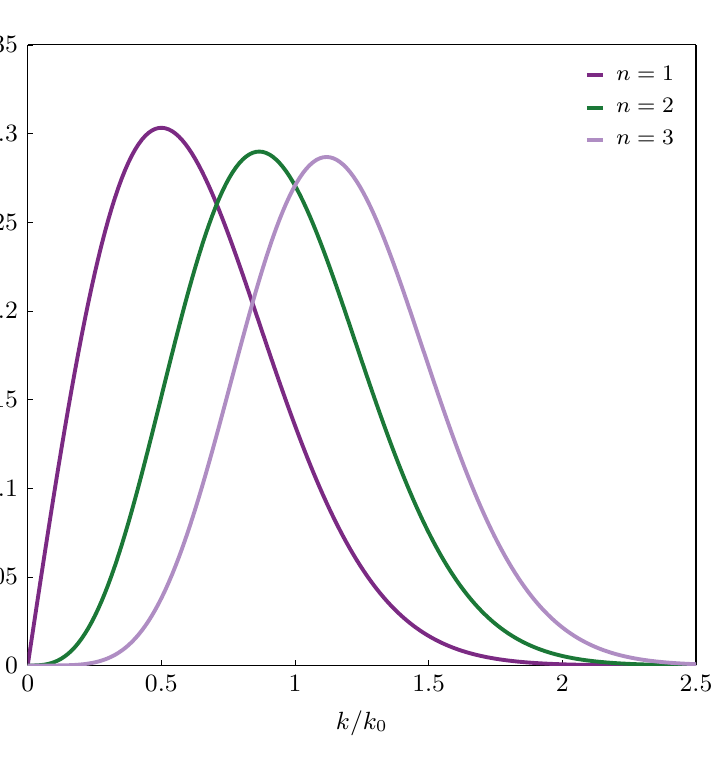
\begin{tikzpicture}[trim axis left,trim axis right]

\begin{axis}[%
width=11.252in,
height=7.131in,
at={(1.887in,0.962in)},
scale only axis,
clip=true,
separate axis lines,
every outer x axis line/.append style={black},
every x tick label/.append style={font=\color{black}},
every x tick/.append style={black},
xmin=0,
xmax=2.5,
xlabel={$k/k_0$},
every outer y axis line/.append style={black},
every y tick label/.append style={font=\color{black}},
every y tick/.append style={black},
ymin=0,
ymax=0.35,
ylabel={$E_{\eta,n}(k)$},
axis background/.style={fill=white},
legend style={legend cell align=left, align=left},
clip=true,
clip mode=individual,
axis lines=box,
xtick pos=bottom,
ytick pos=left,
tick align=inside,
major tick length=2pt,
width=0.7\linewidth,
height=0.65\linewidth,
every axis/.append style={font=\fontsize{9}{9}\selectfont},xlabel style={font=\fontsize{9}{9}\selectfont},title style={font=\fontsize{9}{9}\selectfont},
legend style={font=\fontsize{8}{9}\selectfont,inner sep=1pt,row sep=1pt,column sep=2pt,nodes={scale=1.00},draw=none},legend image post style={xscale=0.35},
legend columns=1,
scaled x ticks=false,
tick label style={/pgf/number format/fixed,/pgf/number format/precision=2},
every x tick label/.append style={font=\fontsize{9}{9}\selectfont\color{black}},
every y tick label/.append style={font=\fontsize{9}{9}\selectfont\color{black}},
,,
colormap={sigmamap}{rgb(0.0000)=(0.0200,0.1880,0.3800); rgb(0.1000)=(0.0743,0.3456,0.5616); rgb(0.2000)=(0.1918,0.4980,0.7060); rgb(0.3000)=(0.3890,0.6708,0.8226); rgb(0.4000)=(0.7552,0.8682,0.9228); rgb(0.5000)=(0.9690,0.9689,0.9689); rgb(0.6000)=(0.9425,0.8044,0.7614); rgb(0.7000)=(0.8767,0.4910,0.4020); rgb(0.8000)=(0.7869,0.2866,0.2470); rgb(0.9000)=(0.6186,0.1239,0.1568); rgb(1.0000)=(0.4040,0.0000,0.1220)}
]
\addplot [color=mycolor1, line width=1.4pt]
  table[row sep=crcr]{%
1e-06	9.99999999998e-07\\
0.012507248124062	0.0125033356870642\\
0.0250134962481241	0.0249822151857268\\
0.0375197443721861	0.0374142575081492\\
0.0500259924962481	0.049776227988151\\
0.0625322406203102	0.0620451106388611\\
0.0750384887443722	0.074198179555138\\
0.0875447368684342	0.0862130690507178\\
0.100050984992496	0.0980678422271457\\
0.112557233116558	0.109741057680322\\
0.12506348124062	0.121211834060891\\
0.137569729364682	0.132459912216648\\
0.151326602301151	0.144552237739127\\
0.163832850425213	0.15526980755966\\
0.176339098549275	0.165706455442367\\
0.188845346673337	0.175845062145538\\
0.201351594797399	0.185669401013813\\
0.213857842921461	0.195164180365556\\
0.226364091045523	0.204315081990821\\
0.238870339169585	0.213108795630047\\
0.251376587293647	0.221533049324865\\
0.263882835417709	0.229576635554121\\
0.276389083541771	0.237229433090159\\
0.288895331665833	0.244482424532426\\
0.301401579789895	0.251327709497517\\
0.313907827913957	0.257758513466586\\
0.326414076038019	0.26376919231265\\
0.338920324162081	0.269355232551407\\
0.351426572286143	0.274513247379763\\
0.363932820410205	0.279240968586193\\
0.376439068534267	0.283537234436133\\
0.388945316658329	0.287401973653864\\
0.401451564782391	0.290836185639548\\
0.413957812906453	0.293841917076269\\
0.427714685842921	0.296657016968592\\
0.440220933966983	0.298774103791276\\
0.452727182091046	0.300475402147823\\
0.465233430215107	0.301766937984341\\
0.47773967833917	0.302655615812989\\
0.490245926463232	0.303149177432573\\
0.502752174587294	0.303256158493771\\
0.515258422711356	0.302985843147067\\
0.527764670835418	0.302348217015337\\
0.54027091895948	0.30135391873543\\
0.552777167083542	0.300014190314105\\
0.565283415207604	0.298340826543286\\
0.577789663331666	0.296346123717858\\
0.590295911455728	0.2940428278962\\
0.60280215957979	0.291444082939338\\
0.615308407703852	0.288563378559127\\
0.627814655827914	0.285414498599276\\
0.640320903951976	0.282011469765338\\
0.652827152076038	0.278368511011214\\
0.6653334002001	0.274499983780127\\
0.677839648324162	0.270420343287768\\
0.690345896448224	0.266144091024213\\
0.704102769384692	0.261230433566072\\
0.716609017508754	0.256588445151956\\
0.729115265632816	0.251794604352604\\
0.741621513756878	0.24686313763554\\
0.75412776188094	0.241808100063135\\
0.766634010005002	0.23664333833741\\
0.779140258129065	0.231382455957741\\
0.791646506253126	0.226038780563521\\
0.804152754377189	0.220625333520528\\
0.816659002501251	0.215154801796455\\
0.829165250625313	0.209639512158135\\
0.841671498749375	0.204091407710348\\
0.854177746873437	0.19852202678381\\
0.866683994997499	0.192942484168157\\
0.879190243121561	0.187363454674395\\
0.891696491245623	0.181795159000548\\
0.904202739369685	0.176247351864029\\
0.916708987493747	0.170729312354729\\
0.929215235617809	0.165249836453935\\
0.941721483741871	0.159817231655987\\
0.954227731865933	0.154439313622079\\
0.966733979989995	0.149123404788854\\
0.980490852926463	0.143355662283408\\
0.992997101050525	0.138191618138487\\
1.00550334917459	0.13310916348621\\
1.01800959729865	0.128113622286538\\
1.03051584542271	0.123209845332416\\
1.04302209354677	0.11840221880887\\
1.05552834167084	0.113694674126555\\
1.0680345897949	0.109090698924165\\
1.08054083791896	0.104593349133712\\
1.09304708604302	0.100205262002926\\
1.10555333416708	0.0959286699697512\\
1.11805958229115	0.0917654152852739\\
1.13056583041521	0.0877169652831892\\
1.14307207853927	0.0837844281962175\\
1.15557832666333	0.0799685694225552\\
1.16808457478739	0.0762698281485362\\
1.18059082291146	0.0726883342371032\\
1.19309707103552	0.0692239252954183\\
1.20560331915958	0.0658761638389392\\
1.21810956728364	0.0626443544735069\\
1.2306158154077	0.0595275610214065\\
1.24312206353177	0.0565246235219153\\
1.25687893646823	0.0533512586932931\\
1.2693851845923	0.050582742554742\\
1.28189143271636	0.04792324446996\\
1.29439768084042	0.0453708597065667\\
1.30690392896448	0.0429235422940296\\
1.31941017708854	0.0405791200311605\\
1.33191642521261	0.038335309011414\\
1.34442267333667	0.0361897276348124\\
1.35692892146073	0.0341399100797784\\
1.36943516958479	0.0321833192124766\\
1.38194141770885	0.0303173589154311\\
1.39444766583292	0.028539385821176\\
1.40695391395698	0.0268467204405133\\
1.41946016208104	0.025236657678563\\
1.4319664102051	0.0237064767352062\\
1.44447265832916	0.022253450389725\\
1.45697890645323	0.020874853672428\\
1.46948515457729	0.0195679719288212\\
1.48199140270135	0.0183301082844277\\
1.49449765082541	0.0171585905206906\\
1.50700389894947	0.0160507773744975\\
1.51951014707354	0.015004064275758\\
1.53326702001	0.0139201932227356\\
1.54577326813407	0.0129935043648222\\
1.55827951625813	0.0121201276874942\\
1.57078576438219	0.0112976577428226\\
1.58329201250625	0.0105237469402583\\
1.59579826063032	0.0097961082518346\\
1.60830450875438	0.00911251749448843\\
1.62081075687844	0.00847081521196432\\
1.6333170050025	0.00786890817898354\\
1.64582325312656	0.00730477055043469\\
1.65832950125063	0.00677644467828962\\
1.67083574937469	0.00628204161877771\\
1.68334199749875	0.00581974135207076\\
1.69584824562281	0.00538779273635341\\
1.70835449374687	0.00498451321768748\\
1.72086074187094	0.00460828831653454\\
1.733366989995	0.00425757091118747\\
1.74587323811906	0.00393088033768892\\
1.75837948624312	0.00362680132509161\\
1.77088573436718	0.00334398278414903\\
1.78339198249125	0.00308113646672591\\
1.79589823061531	0.00283703551239094\\
1.80965510355178	0.0025887842603378\\
1.82216135167584	0.00238031932361065\\
1.8346675997999	0.00218716939922618\\
1.84717384792396	0.00200834229180101\\
1.85968009604802	0.00184289856882796\\
1.87218634417209	0.00168994972555733\\
1.88469259229615	0.00154865632932159\\
1.89719884042021	0.00141822615287879\\
1.90970508854427	0.00129791230555245\\
1.92221133666833	0.00118701137017154\\
1.9347175847924	0.00108486155306661\\
1.94722383291646	0.000990840853659224\\
1.95973008104052	0.000904365259492857\\
1.97223632916458	0.000824886971896154\\
1.98474257728864	0.000751892666844868\\
1.99724882541271	0.000684901794997244\\
2.00975507353677	0.00062346492432005\\
2.02226132166083	0.000567162128198694\\
2.03476756978489	0.000515601421434883\\
2.04727381790895	0.000468417246079032\\
2.05978006603302	0.000425269008621212\\
2.07228631415708	0.00038583966967374\\
2.08604318709355	0.000346411460523943\\
2.09854943521761	0.000313856995799808\\
2.11105568334167	0.000284173937835262\\
2.12356193146573	0.000257128211923276\\
2.13606817958979	0.000232502938143593\\
2.14857442771386	0.00021009734700092\\
2.16108067583792	0.000189725746983587\\
2.17358692396198	0.000171216543082732\\
2.18609317208604	0.000154411305167679\\
2.19859942021011	0.00013916388498924\\
2.21110566833417	0.000125339580478016\\
2.22361191645823	0.000112814345917912\\
2.23611816458229	0.000101474046504826\\
2.24862441270635	9.12137557453812e-05\\
2.26113066083042	8.19370941095129e-05\\
2.27363690895448	7.35556073223929e-05\\
2.28614315707854	6.59881826644289e-05\\
2.2986494052026	5.91605016418098e-05\\
2.31115565332666	5.30045273931476e-05\\
2.32366190145073	4.74580252092345e-05\\
2.33616814957479	4.2464114561786e-05\\
2.34867439769885	3.79708510623788e-05\\
2.36243127063532	3.35500659514266e-05\\
2.37493751875938	2.99588643141167e-05\\
2.38744376688344	2.67345922799202e-05\\
2.3999500150075	2.38417517501924e-05\\
2.41245626313157	2.12480587809647e-05\\
2.42496251125563	1.89241760545548e-05\\
2.43746875937969	1.68434651930235e-05\\
2.44997500750375	1.49817576851635e-05\\
2.46248125562781	1.33171432506067e-05\\
2.47498750375188	1.182977451687e-05\\
2.48749375187594	1.05016869373549e-05\\
2.5	9.31663293019668e-06\\
};
\addlegendentry{$n=1$}

\addplot [color=mycolor2, line width=1.4pt]
  table[row sep=crcr]{%
1e-06	1.999999999996e-18\\
0.012507248124062	3.91182500235304e-06\\
0.0250134962481241	3.12614947005987e-05\\
0.0375197443721861	0.000105338436566632\\
0.0500259924962481	0.000249139968883221\\
0.0625322406203102	0.000485227649066178\\
0.0750384887443722	0.000835586478256945\\
0.0875447368684342	0.00132148788088522\\
0.100050984992496	0.00196335734967166\\
0.112557233116558	0.00278064761171072\\
0.12506348124062	0.00379171813014021\\
0.137569729364682	0.00501372170881961\\
0.151326602301151	0.00662041748434639\\
0.163832850425213	0.00833525681121348\\
0.176339098549275	0.0103054427723424\\
0.188845346673337	0.0125421719033817\\
0.201351594797399	0.0150549902831408\\
0.213857842921461	0.0178517366579682\\
0.226364091045523	0.02093849634428\\
0.238870339169585	0.0243195661344885\\
0.251376587293647	0.0279974303533997\\
0.263882835417709	0.0319727481335621\\
0.276389083541771	0.036244351899698\\
0.288895331665833	0.0408092569748465\\
0.301401579789895	0.0456626821448074\\
0.313907827913957	0.0507980809434863\\
0.326414076038019	0.056207183350368\\
0.338920324162081	0.0618800475231208\\
0.351426572286143	0.0678051211237688\\
0.363932820410205	0.0739693117364142\\
0.376439068534267	0.0803580658185823\\
0.388945316658329	0.0869554555772692\\
0.401451564782391	0.0937442731150242\\
0.413957812906453	0.100706131151188\\
0.427714685842921	0.108540781846169\\
0.440220933966983	0.115801538607845\\
0.452727182091046	0.123172019498758\\
0.465233430215107	0.130630166447205\\
0.47773967833917	0.138153330169548\\
0.490245926463232	0.145718394385814\\
0.502752174587294	0.153301901038872\\
0.515258422711356	0.160880175717106\\
0.527764670835418	0.168429452494566\\
0.54027091895948	0.175925997422113\\
0.552777167083542	0.183346229927788\\
0.565283415207604	0.190666841414204\\
0.577789663331666	0.197864910374866\\
0.590295911455728	0.204918013389573\\
0.60280215957979	0.211804331401061\\
0.615308407703852	0.218502750720376\\
0.627814655827914	0.224992958256707\\
0.640320903951976	0.231255530518063\\
0.652827152076038	0.237272015981847\\
0.6653334002001	0.243025010488528\\
0.677839648324162	0.248498225366866\\
0.690345896448224	0.253676548054941\\
0.704102769384692	0.259015570360991\\
0.716609017508754	0.263530950488702\\
0.729115265632816	0.267712591193295\\
0.741621513756878	0.271550670738605\\
0.75412776188094	0.275036731399896\\
0.766634010005002	0.278163692429428\\
0.779140258129065	0.280925855405849\\
0.791646506253126	0.283318902153342\\
0.804152754377189	0.285339885459202\\
0.816659002501251	0.286987212858155\\
0.829165250625313	0.288260623788246\\
0.841671498749375	0.289161160456131\\
0.854177746873437	0.289691132779161\\
0.866683994997499	0.289854077797518\\
0.879190243121561	0.28965471397187\\
0.891696491245623	0.289098890800455\\
0.904202739369685	0.288193534204232\\
0.916708987493747	0.286946588139744\\
0.929215235617809	0.285366952906717\\
0.941721483741871	0.283464420621233\\
0.954227731865933	0.281249608325641\\
0.966733979989995	0.278733889203472\\
0.980490852926463	0.275633462054939\\
0.992997101050525	0.272525822525016\\
1.00550334917459	0.269156574707533\\
1.01800959729865	0.265539449734544\\
1.03051584542271	0.261688571204898\\
1.04302209354677	0.25761838441254\\
1.05552834167084	0.253343586669873\\
1.0680345897949	0.248879059071574\\
1.08054083791896	0.244239800020315\\
1.09304708604302	0.239440860810677\\
1.10555333416708	0.234497283541543\\
1.11805958229115	0.229424041600589\\
1.13056583041521	0.224235982937377\\
1.14307207853927	0.218947776314266\\
1.15557832666333	0.213573860697076\\
1.16808457478739	0.208128397920342\\
1.18059082291146	0.202625228735368\\
1.19309707103552	0.197077832323188\\
1.20560331915958	0.191499289329223\\
1.21810956728364	0.18590224845199\\
1.2306158154077	0.18029889659484\\
1.24312206353177	0.17470093256743\\
1.25687893646823	0.168562732150052\\
1.2693851845923	0.163011866002044\\
1.28189143271636	0.157499325565096\\
1.29439768084042	0.152034607235555\\
1.30690392896448	0.146626638441337\\
1.31941017708854	0.141283771586688\\
1.33191642521261	0.136013780932139\\
1.34442267333667	0.130823862268147\\
1.35692892146073	0.125720635232066\\
1.36943516958479	0.120710148110709\\
1.38194141770885	0.115797884964886\\
1.39444766583292	0.110988774907839\\
1.40695391395698	0.106287203366435\\
1.41946016208104	0.101697025152242\\
1.4319664102051	0.0972215791690861\\
1.44447265832916	0.092863704584415\\
1.45697890645323	0.0886257582935311\\
1.46948515457729	0.084509633508598\\
1.48199140270135	0.0805167793080312\\
1.49449765082541	0.0766482209864793\\
1.50700389894947	0.0729045810509312\\
1.51951014707354	0.0692861007145002\\
1.53326702001	0.0654501803871208\\
1.54577326813407	0.0620937483722139\\
1.55827951625813	0.0588610377416395\\
1.57078576438219	0.0557509565170094\\
1.58329201250625	0.052762143839635\\
1.59579826063032	0.0498929917026545\\
1.60830450875438	0.0471416663392376\\
1.62081075687844	0.0445061291813547\\
1.6333170050025	0.0419841573119727\\
1.64582325312656	0.0395733633418135\\
1.65832950125063	0.0372712146499506\\
1.67083574937469	0.0350750519354708\\
1.68334199749875	0.0329821070351399\\
1.69584824562281	0.0309895199694631\\
1.70835449374687	0.0290943551866689\\
1.72086074187094	0.0272936169809641\\
1.733366989995	0.0255842640678607\\
1.74587323811906	0.0239632233054625\\
1.75837948624312	0.0224274025562953\\
1.77088573436718	0.020973702689564\\
1.78339198249125	0.0195990287286103\\
1.79589823061531	0.0183003001528321\\
1.80965510355178	0.0169557685220001\\
1.82216135167584	0.0158066151622171\\
1.8346675997999	0.0147240471498316\\
1.84717384792396	0.0137051335517257\\
1.85968009604802	0.0127469978986512\\
1.87218634417209	0.0118468237386303\\
1.88469259229615	0.0110018595047996\\
1.89719884042021	0.0102094227289079\\
1.90970508854427	0.00946690363279301\\
1.92221133666833	0.0087717681309781\\
1.9347175847924	0.00812156027807352\\
1.94722383291646	0.0075139041949537\\
1.95973008104052	0.00694650550772695\\
1.97223632916458	0.00641715233334719\\
1.98474257728864	0.00592371584535152\\
1.99724882541271	0.00546415045266323\\
2.00975507353677	0.00503649362369966\\
2.02226132166083	0.00463886538718285\\
2.03476756978489	0.0042694675400896\\
2.04727381790895	0.003926582592112\\
2.05978006603302	0.00360857247484645\\
2.07228631415708	0.00331387704270614\\
2.08604318709355	0.00301487171909493\\
2.09854943521761	0.00276439575655084\\
2.11105568334167	0.00253287419120097\\
2.12356193146573	0.00231904719951338\\
2.13606817958979	0.00212172289180142\\
2.14857442771386	0.00193977504995146\\
2.16108067583792	0.00177214081014392\\
2.17358692396198	0.00161781830665559\\
2.18609317208604	0.00147586429152291\\
2.19859942021011	0.00134539174357198\\
2.21110566833417	0.0012255674790868\\
2.22361191645823	0.00111560977519774\\
2.23611816458229	0.00101478601593084\\
2.24862441270635	0.00092241036976801\\
2.26113066083042	0.000837841506531585\\
2.27363690895448	0.000760480360424915\\
2.28614315707854	0.0006897679451351\\
2.2986494052026	0.00062518322603573\\
2.31115565332666	0.000566241053715621\\
2.32366190145073	0.000512490162304697\\
2.33616814957479	0.000463511235369099\\
2.34867439769885	0.00041891504150344\\
2.36243127063532	0.000374491305379288\\
2.37493751875938	0.000337955655540948\\
2.38744376688344	0.000304768349542068\\
2.3999500150075	0.000274645539675444\\
2.41245626313157	0.000247325076337819\\
2.42496251125563	0.000222565084071919\\
2.43746875937969	0.00020014260831892\\
2.44997500750375	0.00017985233160018\\
2.46248125562781	0.000161505357616685\\
2.47498750375188	0.000144928061558302\\
2.48749375187594	0.000129961004750119\\
2.5	0.000116457911627458\\
};
\addlegendentry{$n=2$}

\addplot [color=mycolor3, line width=1.4pt]
  table[row sep=crcr]{%
1e-06	1.999999999996e-30\\
0.012507248124062	6.11931696949723e-10\\
0.0250134962481241	1.95595355265756e-08\\
0.0375197443721861	1.48288205584267e-07\\
0.0500259924962481	6.23497667500118e-07\\
0.0625322406203102	1.89737651358801e-06\\
0.0750384887443722	4.70499927917366e-06\\
0.0875447368684342	1.01279900979929e-05\\
0.100050984992496	1.96535989523522e-05\\
0.112557233116558	3.5228388098081e-05\\
0.12506348124062	5.930578680631e-05\\
0.137569729364682	9.48868414331085e-05\\
0.151326602301151	0.000151605842816972\\
0.163832850425213	0.000223728319113764\\
0.176339098549275	0.000320452665680735\\
0.188845346673337	0.000447286020246002\\
0.201351594797399	0.000610366412526424\\
0.213857842921461	0.000816452335435037\\
0.226364091045523	0.00107290324553506\\
0.238870339169585	0.0013876510709499\\
0.251376587293647	0.0017691629054498\\
0.263882835417709	0.00222639516592098\\
0.276389083541771	0.00276873958580403\\
0.288895331665833	0.00340596150832547\\
0.301401579789895	0.00414813102945641\\
0.313907827913957	0.00500554762059392\\
0.326414076038019	0.00598865893412824\\
0.338920324162081	0.00710797456057011\\
0.351426572286143	0.0083739755630968\\
0.363932820410205	0.00979702066366017\\
0.376439068534267	0.0113872499937184\\
0.388945316658329	0.0131544873518456\\
0.401451564782391	0.0151081419296906\\
0.413957812906453	0.0172571104768691\\
0.427714685842921	0.0198564346196217\\
0.440220933966983	0.022441697881073\\
0.452727182091046	0.0252455713162482\\
0.465233430215107	0.0282738733739445\\
0.47773967833917	0.0315314529777793\\
0.490245926463232	0.0350221145942289\\
0.502752174587294	0.0387485500358184\\
0.515258422711356	0.0427122776924657\\
0.527764670835418	0.0469135898131991\\
0.54027091895948	0.0513515083839636\\
0.552777167083542	0.0560237500658531\\
0.565283415207604	0.0609267005727671\\
0.577789663331666	0.066055398779111\\
0.590295911455728	0.0714035307576907\\
0.60280215957979	0.0769634338563467\\
0.615308407703852	0.0827261108300827\\
0.627814655827914	0.0886812539544072\\
0.640320903951976	0.0948172789562263\\
0.652827152076038	0.101121368511796\\
0.6653334002001	0.107579524977781\\
0.677839648324162	0.114176631942163\\
0.690345896448224	0.120896524107343\\
0.704102769384692	0.128409743025713\\
0.716609017508754	0.135330649484918\\
0.729115265632816	0.142318441786513\\
0.741621513756878	0.149353539545975\\
0.75412776188094	0.156415776806873\\
0.766634010005002	0.163484508648307\\
0.779140258129065	0.170538721072961\\
0.791646506253126	0.177557143330142\\
0.804152754377189	0.184518361818804\\
0.816659002501251	0.191400934713995\\
0.829165250625313	0.19818350646635\\
0.841671498749375	0.204844921337904\\
0.854177746873437	0.211364335158293\\
0.866683994997499	0.217721324513027\\
0.879190243121561	0.223895992609469\\
0.891696491245623	0.229869071106017\\
0.904202739369685	0.235622017235191\\
0.916708987493747	0.241137105601301\\
0.929215235617809	0.246397514087601\\
0.941721483741871	0.251387403365527\\
0.954227731865933	0.25609198955938\\
0.966733979989995	0.26049760968273\\
0.980490852926463	0.264983622531054\\
0.992997101050525	0.26872224576062\\
1.00550334917459	0.272127251839416\\
1.01800959729865	0.275190093398575\\
1.03051584542271	0.277903555980051\\
1.04302209354677	0.280261774884728\\
1.05552834167084	0.282260243937691\\
1.0680345897949	0.283895816303325\\
1.08054083791896	0.285166697538785\\
1.09304708604302	0.286072431126841\\
1.10555333416708	0.286613876777935\\
1.11805958229115	0.286793181836096\\
1.13056583041521	0.286613746163924\\
1.14307207853927	0.286080180917951\\
1.15557832666333	0.285198261657216\\
1.16808457478739	0.283974876254653\\
1.18059082291146	0.282417968102941\\
1.19309707103552	0.280536475123704\\
1.20560331915958	0.278340265101477\\
1.21810956728364	0.275840067871729\\
1.2306158154077	0.273047404895582\\
1.24312206353177	0.269974516752834\\
1.25687893646823	0.266286076147086\\
1.2693851845923	0.262667335887439\\
1.28189143271636	0.258810080868057\\
1.29439768084042	0.254728717361335\\
1.30690392896448	0.250437987542292\\
1.31941017708854	0.24595289521349\\
1.33191642521261	0.241288632862561\\
1.34442267333667	0.236460510444566\\
1.35692892146073	0.231483886252473\\
1.36943516958479	0.226374100208726\\
1.38194141770885	0.221146409879324\\
1.39444766583292	0.21581592947951\\
1.40695391395698	0.210397572107358\\
1.41946016208104	0.204905995408433\\
1.4319664102051	0.199355550841804\\
1.44447265832916	0.193760236684988\\
1.45697890645323	0.188133654883479\\
1.46948515457729	0.182488971819262\\
1.48199140270135	0.176838883042654\\
1.49449765082541	0.171195581982911\\
1.50700389894947	0.165570732625596\\
1.51951014707354	0.159975446118827\\
1.53326702001	0.153867336615347\\
1.54577326813407	0.148367733548091\\
1.55827951625813	0.142928434970103\\
1.57078576438219	0.137558121484787\\
1.58329201250625	0.132264859577002\\
1.59579826063032	0.127056100088265\\
1.60830450875438	0.121938679765726\\
1.62081075687844	0.116918825705802\\
1.6333170050025	0.112002162504847\\
1.64582325312656	0.107193721922586\\
1.65832950125063	0.102497954859222\\
1.67083574937469	0.0979187454440442\\
1.68334199749875	0.0934594270319558\\
1.69584824562281	0.0891227999044873\\
1.70835449374687	0.0849111504734621\\
1.72086074187094	0.0808262717884554\\
1.733366989995	0.0768694851533864\\
1.74587323811906	0.0730416626629076\\
1.75837948624312	0.0693432504755988\\
1.77088573436718	0.0657742926481854\\
1.78339198249125	0.0623344553630029\\
1.79589823061531	0.0590230513895659\\
1.80965510355178	0.0555276255685623\\
1.82216135167584	0.0524822616041784\\
1.8346675997999	0.0495612192972269\\
1.84717384792396	0.0467626177164741\\
1.85968009604802	0.0440843457628693\\
1.87218634417209	0.0415240851759331\\
1.88469259229615	0.0390793329261024\\
1.89719884042021	0.0367474229148731\\
1.90970508854427	0.0345255469145283\\
1.92221133666833	0.0324107746889247\\
1.9347175847924	0.0304000732461812\\
1.94722383291646	0.0284903251831199\\
1.95973008104052	0.0266783460899086\\
1.97223632916458	0.0249609009915164\\
1.98474257728864	0.0233347198102868\\
1.99724882541271	0.0217965118411319\\
2.00975507353677	0.0203429792375503\\
2.02226132166083	0.0189708295128481\\
2.03476756978489	0.0176767870665974\\
2.04727381790895	0.0164576037515019\\
2.05978006603302	0.0153100685004512\\
2.07228631415708	0.014231016037647\\
2.08604318709355	0.0131194439538038\\
2.09854943521761	0.0121741493755179\\
2.11105568334167	0.011287895922692\\
2.12356193146573	0.0104577787737574\\
2.13606817958979	0.00968097019663025\\
2.14857442771386	0.00895472336544476\\
2.16108067583792	0.00827637550756156\\
2.17358692396198	0.00764335042112507\\
2.18609317208604	0.00705316040372525\\
2.19859942021011	0.00650340763270439\\
2.21110566833417	0.0059917850373634\\
2.22361191645823	0.00551607670279081\\
2.23611816458229	0.00507415784429085\\
2.24862441270635	0.0046639943904439\\
2.26113066083042	0.00428364221172457\\
2.27363690895448	0.00393124603034815\\
2.28614315707854	0.00360503804564062\\
2.2986494052026	0.00330333630775216\\
2.31115565332666	0.00302454287097773\\
2.32366190145073	0.00276714175633238\\
2.33616814957479	0.0025296967513686\\
2.34867439769885	0.00231084907353713\\
2.36243127063532	0.00209006649953723\\
2.37493751875938	0.001906180820384\\
2.38744376688344	0.00173714537910419\\
2.3999500150075	0.00158189241407161\\
2.41245626313157	0.00143941839619503\\
2.42496251125563	0.00130878133095834\\
2.43746875937969	0.0011890980628289\\
2.44997500750375	0.00107954159524468\\
2.46248125562781	0.00097933843798312\\
2.47498750375188	0.000887765992373468\\
2.48749375187594	0.000804149983541334\\
2.5	0.000727861947671615\\
};
\addlegendentry{$n=3$}

\node[overlay,right, align=left, inner sep=0]
at (rel axis cs:-0.15,1.1) {$(b)$};
\end{axis}
\end{tikzpicture}%
    \end{minipage}
    \caption{Two-dimensional isotropic spectra and correlations for the first three members of the family defined in \eqref{eq:eta_spectrum_family} and
    \eqref{eq:eta_correlation_family}. (a) Physical-space correlation function
    \(C_{00,n}^{xy}(r)\).
    (b) Corresponding two-dimensional isotropic wavenumber spectrum \(E_{\eta,n}(k)\).}
    \label{fig:eta_2d_family}
\end{figure}
To make this connection explicit, consider the family of isotropic spectra
\begin{equation}
    E_{\eta,n}(k)
    =
    \frac{2^n\mean{\eta_0^2}}{(n-1)!\,k_0}
    \left(\frac{k}{k_0}\right)^{2n-1}
    \exp\!\left[
        -2\left(\frac{k}{k_0}\right)^2
    \right],
    \qquad
    n=1,2,\ldots,
    \label{eq:eta_spectrum_family}
\end{equation}
where \(k_0\) is the characteristic horizontal wavenumber of the perturbation field. Applying \eqref{eq:eta_hankel_transform_pair} gives the corresponding isotropic correlation function
\begin{equation}
    C_{00,n}^{xy}(r)
    =
    \mean{\eta_0^2}
    \exp\!\left(-\frac{k_0^2 r^2}{8}\right)
    L_{n-1}^{(0)}
    \!\left(
        \frac{k_0^2 r^2}{8}
    \right),
    \label{eq:eta_correlation_family}
\end{equation}
where \(L_n^{(0)}\) denotes the Laguerre polynomial of degree \(n\) and order zero. \Cref{fig:eta_2d_family} shows the spectrum \(E_{\eta,n}(k)\) together with its physical-space counterpart \(C_{00,n}^{xy}(r)\) for the first three members of this family. Defining the reference length scale
\begin{equation}
    \lambda_0
    =
    \frac{2\sqrt{2}}{k_0},
    \label{eq:lambda0_k0_relation}
\end{equation}
the first three correlations are
\begin{equation}
\begin{aligned}
    C_{00,1}^{xy}(r)
    &=
    \mean{\eta_0^2}
    \exp\!\left(-\frac{r^2}{\lambda_0^2}\right),
    \\
    C_{00,2}^{xy}(r)
    &=
    \mean{\eta_0^2}
    \left(
        1-\frac{r^2}{\lambda_0^2}
    \right)
    \exp\!\left(-\frac{r^2}{\lambda_0^2}\right),
    \\
    C_{00,3}^{xy}(r)
    &=
    \mean{\eta_0^2}
    \left(
        1
        -
        2\frac{r^2}{\lambda_0^2}
        +
        \frac{1}{2}\frac{r^4}{\lambda_0^4}
    \right)
    \exp\!\left(-\frac{r^2}{\lambda_0^2}\right).
\end{aligned}
\label{eq:eta_correlation_family_examples}
\end{equation}
The first member of this family recovers the Gaussian correlation used by \citet{frame-towne-2024} to describe three-dimensional perturbation growth, but here it is tied directly to a physical quantity through the corresponding spectrum. The higher-order members produce correlations consisting of a Gaussian envelope multiplied by a polynomial, with the corresponding spectra distributing the initial variance differently across the horizontal wavenumbers.

The subsequent analysis is restricted to the family of spectra introduced in \eqref{eq:eta_spectrum_family}, although this choice is not fundamental to the formulation. Whenever either a model for the spectrum or a physical-space correlation is available, the Hankel transform pair in \eqref{eq:eta_hankel_transform_pair} provides the corresponding representation in the other domain; casting the initial statistics in spectral space therefore does more than provide an equivalent description, as it gives the covariance model a direct physical interpretation in terms of an interface perturbation that can be imposed experimentally or numerically. We stress that relaxing the isotropy assumption the same connection can be drawn, however losing the immediate connection that practitioners have with homogeneous-isotropic fields.
